\documentclass{beamer}

\mode<presentation>
{
  \usetheme{Warsaw}
  \useoutertheme{infolines}
  \setbeamercovered{transparent}
}

\usepackage[spanish]{babel}
\usepackage[utf8]{inputenc}
\usepackage[T1]{fontenc}
\usepackage{times}
\usepackage{hyperref}
\usepackage{multicol}
\usepackage{graphicx}
\usepackage{verbatim}
\usepackage{amsmath}
\usepackage{listings}
\usepackage{ulem}
\usepackage{pdfpages}
\usepackage{color, colortbl}

\definecolor{LRed}{rgb}{1,.9,.9}
\definecolor{MRed}{rgb}{1,.6,.6}
\definecolor{HRed}{rgb}{1,.2,.2}

\lstloadlanguages{C++,Python}
\lstset{
  basicstyle=\ttfamily\small,
  numbers=left,
  numberstyle=\tiny,
  stepnumber=1,
  numbersep=9pt,
  frame=l,
  framesep=3pt,
  breaklines=true
}

% ==========================
% Metadatos de la presentación
% ==========================

\title[Similitud de firmas manuscritas]{Similitud de firmas manuscritas, caso práctico para validación automática de documentos electorales.}
\subtitle{Tesina de Grado – Licenciatura en Ciencias de la Computación}
\author[Mariano Crosetti]{Mariano Crosetti\\\texttt{C-5994/3}}
\institute[UNR]{Universidad Nacional de Rosario\\[0.5em] Rosario, Argentina\\[0.5em] Director: Dante Zanarini\\Co-director: Pablo Granitto}
\date[Defensa de Tesina]{31 de diciembre de 2024}

% ==========================
% Tabla de contenidos por subsección
% ==========================

\AtBeginSubsection[]
{
  \begin{frame}{Contenidos}
    \footnotesize
    \tableofcontents[currentsection, currentsubsection]
  \end{frame}
}

\begin{document}

% ==========================
% Portada y contenidos
% ==========================

\begin{frame}
  \titlepage
\end{frame}

\begin{frame}{Contenidos}
  \tableofcontents
\end{frame}

% ==========================
% Sección 1: Introducción y contexto personal
% ==========================

\section{Introducción y contexto}

\begin{frame}{Quién soy y qué hago}
  \begin{itemize}
    \item Trabajo en \textbf{Machine Learning} y \textbf{Visión Computarizada} hace varios años.
    \item Vengo del mundo de la matemática / computación y terminé cayendo en ML (como muchos físicos y matemáticos, porque es \textbf{muy divertido}).
    \item Hacer ML en la vida real no es sólo ``entrenar modelos'': hay que \textbf{saber programar}, armar datos, depurar, automatizar.
    \item Esta tesina es un ejemplo concreto de un problema real abordado con herramientas modernas de ML.
  \end{itemize}
\end{frame}

\begin{frame}{De qué va esta charla}
  \begin{itemize}
    \item Contar \textbf{qué problema real} estuvimos resolviendo con ML: firmas en telegramas electorales.
    \item Aprovechar para explicar con intuiciones qué es lo que hago cuando ``trabajo en ML''.
    \item Mostrar \textbf{un camino completo}: desde el dato crudo hasta los modelos y resultados.
    \item Compartir algunas opiniones personales:
      \begin{itemize}
        \item La jerga de DL es \textbf{innecesariamente enrevesada}.
        \item ``Ciencia negativa'': cuánto se puede perder por un bug.
        \item Consejo de oro: \textbf{visualizar los resultados todo el tiempo}.
      \end{itemize}
  \end{itemize}
\end{frame}

% ==========================
% Sección 2: ML y redes neuronales — intuiciones
% ==========================

\section{ML y redes neuronales}

\begin{frame}{Qué es ML (versión no académica)}
  \begin{itemize}
    \item Queremos que una computadora aprenda una función \( f(x) \) a partir de ejemplos en vez de programarla a mano.
    \item En visión por computadora: \( x \) es una imagen y \( f(x) \) puede ser ``hay firma / no hay firma'' o ``estas dos firmas coinciden''.
    \item El modelo es una \textbf{gran composición de capas} con parámetros que vamos ajustando.
    \item Aprender = ajustar esos parámetros para que las predicciones se parezcan a la realidad en los datos de entrenamiento.
  \end{itemize}
\vfill
\begin{center}
  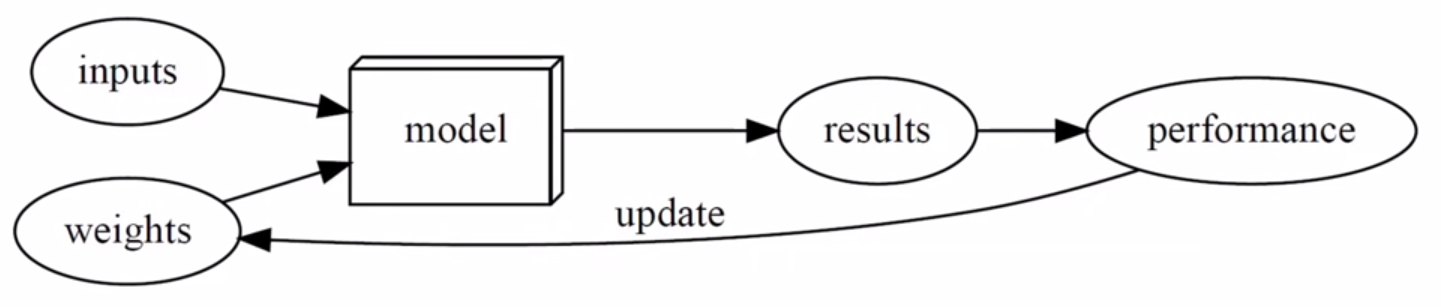
\includegraphics[width=0.7\textwidth]{../latex-informe/imgs/automated-learning.png}
\end{center}
\end{frame}

\begin{frame}{Intuición de una red neuronal}
  \begin{itemize}
    \item Pensar una red como una \textbf{tubería de procesamiento} de la imagen.
    \item Capas iniciales: detectan bordes y trazos simples.
    \item Capas intermedias: combinan trazos en formas más complejas.
    \item Capas finales: resumen todo en un vector (\emph{embedding}) que captura el estilo de la firma.
    \item Dos firmas del mismo autor deberían quedar cerca en ese espacio; de autores distintos, lejos.
  \end{itemize}
\vfill
\begin{center}
  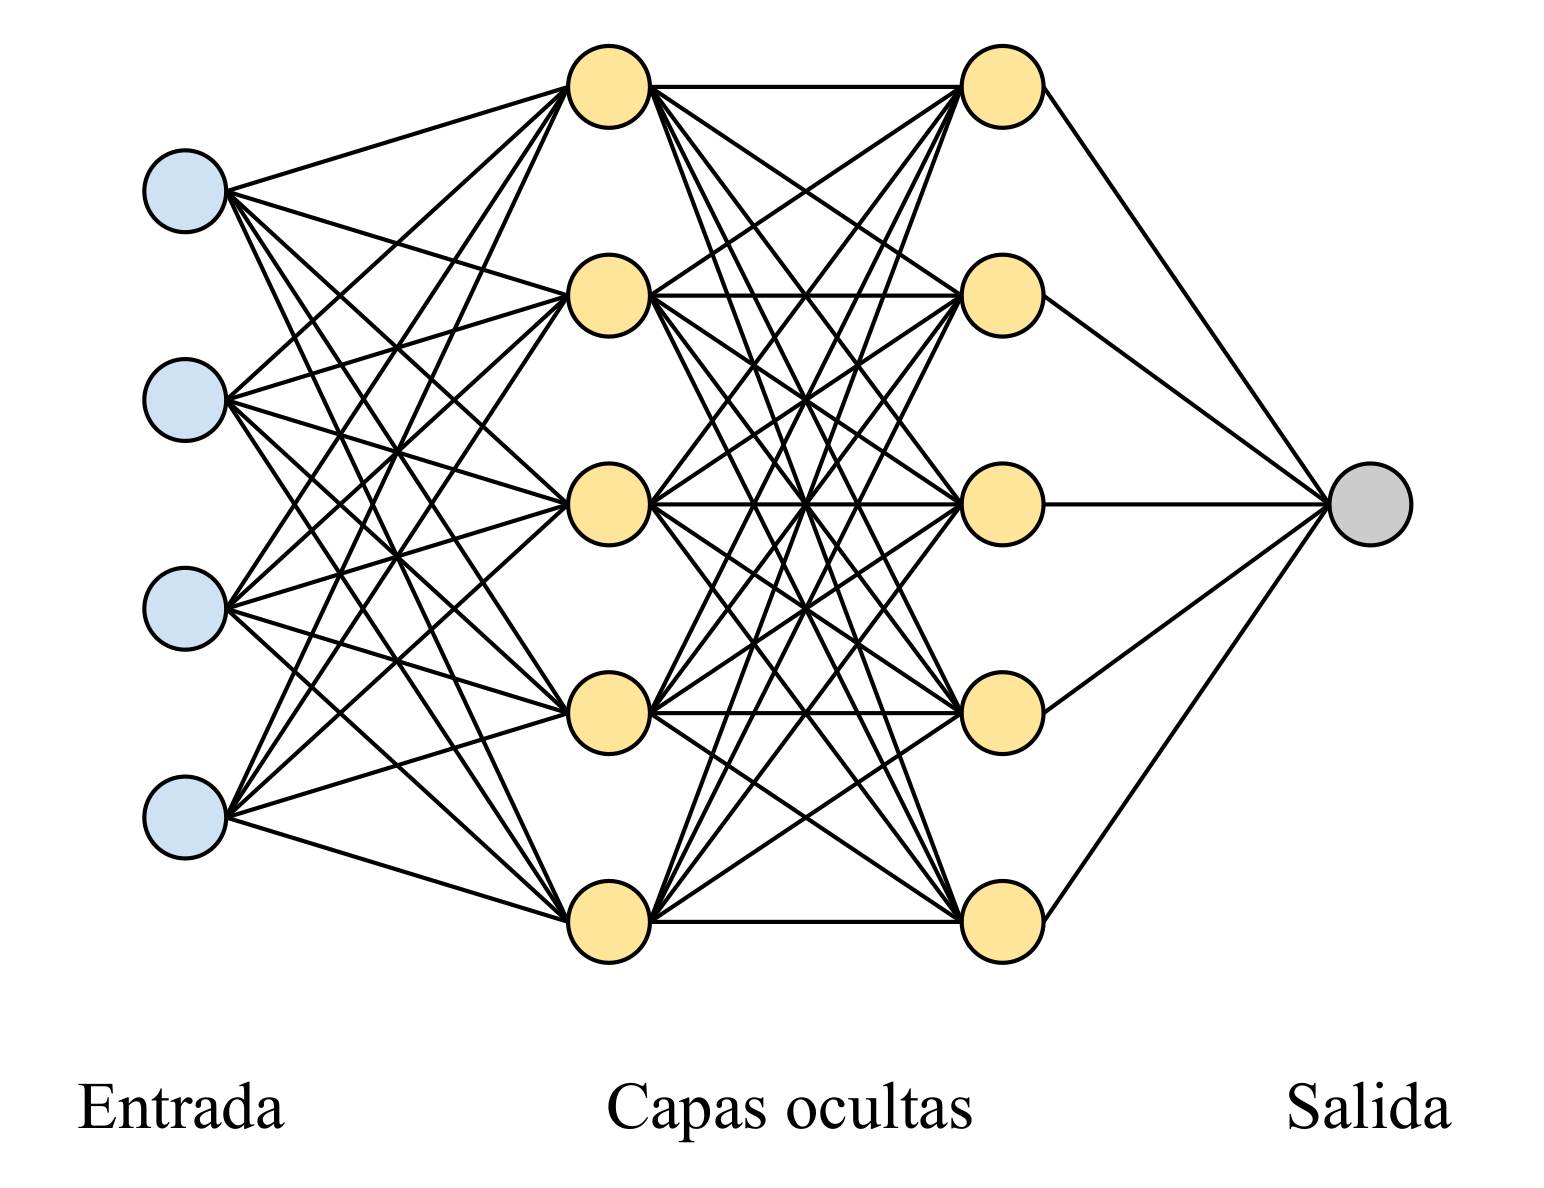
\includegraphics[width=0.7\textwidth]{../latex-informe/imgs/feedforward.png}
\end{center}
\end{frame}

\begin{frame}{Aprendizaje supervisado y pérdida}
  \begin{itemize}
    \item Tenemos pares de entrada–salida \((x, y)\) donde \(y\) indica si dos firmas coinciden o no.
    \item Definimos una \textbf{función de pérdida} que penaliza mucho los errores importantes.
    \item Optimizamos para \textbf{minimizar} esa pérdida en los datos de entrenamiento.
    \item En la tesina, la métrica clave no es el ``accuracy'' sino:
      \begin{itemize}
        \item Maximizar la \textit{precision} con \textit{recall} \(\geq 0{,}9\).
      \end{itemize}
  \end{itemize}
\end{frame}

% ==========================
% Sección 3: Problema y contexto electoral
% ==========================

\section{El problema de las firmas en telegramas}

\begin{frame}{Contexto electoral}
  \begin{itemize}
    \item Proyecto dentro del escrutinio provisorio asistido digitalmente de la Provincia de Santa Fe.
    \item Sistemas como SETT y SIAAM ya asisten la transmisión y carga de telegramas.
    \item Aun así hay \textbf{retransmisiones}: errores de confección que generan trabajo extra.
    \item Idea: sumar chequeos automáticos tempranos para reducir ese trabajo y mejorar la velocidad del escrutinio.
  \end{itemize}
\end{frame}

\begin{frame}{Telegramas electorales}
  \begin{itemize}
    \item Documentos que resumen los votos de una mesa, con formato fijo conocido de antemano.
    \item Se escanean/fotografían y se envían al centro de cómputo.
    \item Deben estar \textbf{firmados en todas las páginas} por las autoridades de mesa.
    \item Problemas típicos: firmas faltantes, en casilleros equivocados o en páginas incompletas.
  \end{itemize}
\vfill
\begin{center}
  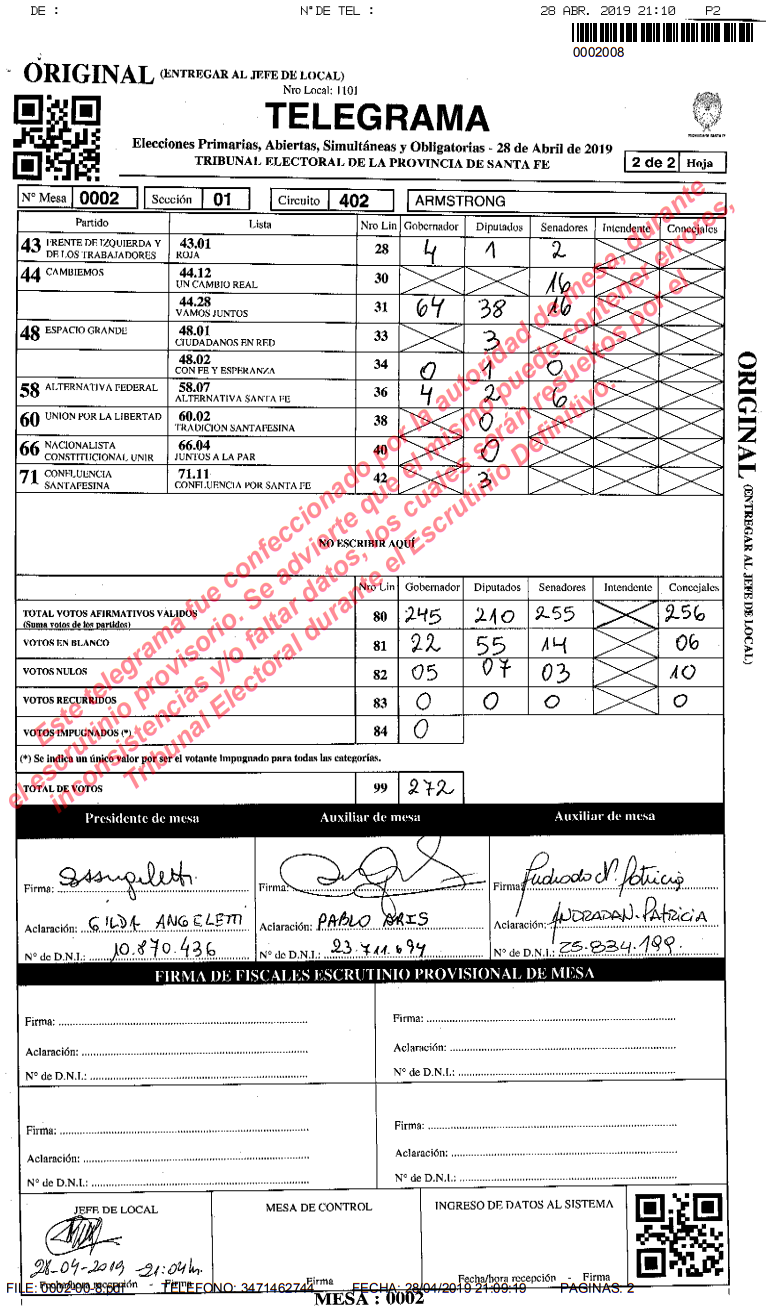
\includegraphics[width=0.7\textwidth]{../latex-informe/imgs/telegramas1.png}
\end{center}
\end{frame}

\begin{frame}{Objetivo de la tesina}
  \begin{itemize}
    \item Enfocarnos en el chequeo de \textbf{firmas manuscritas}:
      \begin{itemize}
        \item Detectar si la firma está presente donde debería.
        \item Verificar si firmas de distintas páginas del mismo telegrama coinciden.
      \end{itemize}
    \item No buscamos falsificaciones artísticas, sino \textbf{errores de confección} del telegrama.
    \item Formalmente: decidir si dos recortes de firma son del mismo autor o no.
  \end{itemize}
\end{frame}

% ==========================
% Sección 4: Datos y construcción del dataset
% ==========================

\section{Datos y construcción del dataset}

\begin{frame}{Datasets de firmas existentes}
  \begin{itemize}
    \item \textbf{CEDAR Signature}: firmas auténticas y falsificaciones de varios autores.
    \item \textbf{SigComp 2009}: dataset diseñado para competencias de verificación de firmas.
    \item Los adaptamos a nuestro problema:
      \begin{itemize}
        \item Usamos principalmente firmas auténticas.
        \item Generamos pares positivos (mismo autor) y negativos (autores distintos).
      \end{itemize}
  \end{itemize}
\end{frame}

\begin{frame}{Construyendo un dataset propio}
  \begin{itemize}
    \item Partimos de \textbf{imágenes completas de telegramas}.
    \item Como la estructura del formulario es fija, recortamos las zonas donde deberían ir las firmas.
    \item Para decidir si hay o no hay firma:
      \begin{itemize}
        \item Primero una heurística simple con componentes conexas (\(\sim 0{,}90\) de \textit{accuracy}).
        \item Luego un clasificador neuronal pequeño que alcanza \(\sim 0{,}99\) de \textit{accuracy}.
      \end{itemize}
    \item El modelo se usa como herramienta para \textbf{limpiar y etiquetar} el dataset propio.
  \end{itemize}
\vfill
\begin{center}
  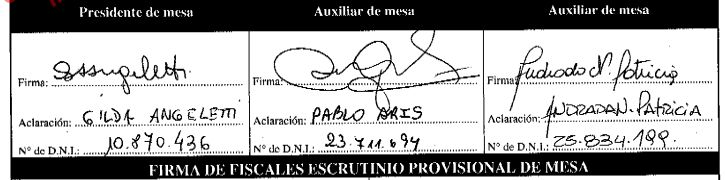
\includegraphics[width=0.7\textwidth]{../latex-informe/imgs/telegramas2.png}
\end{center}
\end{frame}

\begin{frame}{Ciencia negativa y bugs en ML}
  \begin{itemize}
    \item Un bug en extracción o etiquetado de datos puede arruinar semanas de entrenamiento.
    \item Muchas ``malas ideas'' en ML son en realidad \textbf{buenas ideas con un bug}.
    \item Lecciones:
      \begin{itemize}
        \item Visualizar los datos y resultados \textbf{todo el tiempo}.
        \item No confiar ciegamente en que el código hace exactamente lo que dice el paper.
      \end{itemize}
  \end{itemize}
\end{frame}

% ==========================
% Sección 5: Modelos y experimentos
% ==========================

\section{Modelos y experimentos}

\begin{frame}{Enfoque clásico vs Deep Learning}
  \begin{itemize}
    \item \textbf{Enfoque clásico} (inspirado en Parodi):
      \begin{itemize}
        \item Features manuales sobre grillas de la imagen.
        \item Clasificadores tipo Random Forest / SVM.
      \end{itemize}
    \item \textbf{Redes siamesas}:
      \begin{itemize}
        \item Aprenden directamente un embedding a partir de píxeles.
        \item Comparan firmas midiendo distancia en el espacio de embeddings.
      \end{itemize}
    \item Comparamos ambos enfoques en datasets estándar y en el dataset propio.
  \end{itemize}
\end{frame}

\begin{frame}{Redes siamesas y triplet loss}
  \begin{itemize}
    \item Dos ramas comparten pesos y producen \(G_W(\text{firmaA})\) y \(G_W(\text{firmaB})\).
    \item Entrenamos con pares (coinciden / no coinciden) y con \textit{triplet loss}.
    \item Intuición: agrupar firmas del mismo autor y alejar firmas de autores distintos en el espacio de embeddings.
  \end{itemize}
\vfill
\begin{center}
  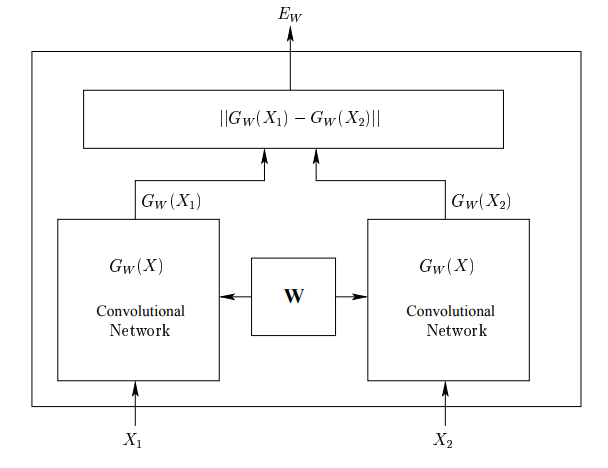
\includegraphics[width=0.7\textwidth]{../latex-informe/imgs/siamess.png}
\end{center}
\end{frame}

\begin{frame}{Métricas de evaluación}
  \begin{itemize}
    \item Métrica principal: \textbf{máxima precision con recall \(\geq 0{,}9\)}.
    \item Interpretación práctica:
      \begin{itemize}
        \item Capturar al menos el 90\% de errores de firmas no coincidentes.
        \item Que la mayoría de las alarmas que emitimos sean problemas reales.
      \end{itemize}
    \item Usamos curvas ROC y Precision–Recall para comparar variantes de modelo.
  \end{itemize}
\vfill
\begin{center}
  \begin{columns}
    \begin{column}{0.48\textwidth}
      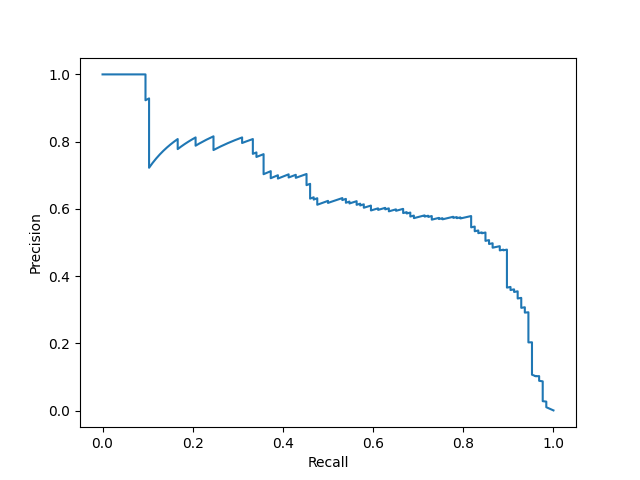
\includegraphics[width=\textwidth]{../latex-informe/imgs/precisionrecall.png}
    \end{column}
    \begin{column}{0.48\textwidth}
      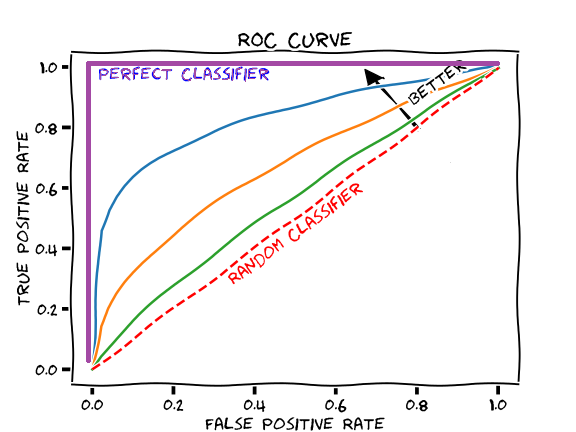
\includegraphics[width=\textwidth]{../latex-informe/imgs/roccurve.png}
    \end{column}
  \end{columns}
\end{center}
\end{frame}

% ==========================
% Sección 6: Conclusiones y trabajo futuro
% ==========================

\section{Conclusiones y trabajo futuro}

\begin{frame}{Qué me llevo de esta tesina}
  \begin{itemize}
    \item Un caso claro de cómo aplicar ML a un problema real y delicado en contexto electoral.
    \item Que el \textbf{pipeline de datos} es tan importante como la arquitectura del modelo.
    \item La importancia de comparar con soluciones previas y construir buenos baselines.
    \item Que una tesina individual enseña tanto de \textbf{gestionar un proyecto} como de teoría.
  \end{itemize}
\end{frame}

\begin{frame}{Trabajo futuro}
  \begin{itemize}
    \item Extender el sistema hacia \textbf{detección de suplantaciones}, no sólo errores de confección.
    \item Integrar el módulo de firmas con más chequeos automáticos del telegrama (números, totales, etc.).
    \item Explorar arquitecturas más modernas de visión (por ejemplo, Transformers para imágenes).
  \end{itemize}
\end{frame}

% ==========================
% Sección 7: Preguntas
% ==========================

\section*{Preguntas}

\begin{frame}{Preguntas}
  \centering
  \vfill
  \textbf{Preguntas, comentarios y chismes de ML bienvenidos}
  \vfill
\end{frame}

% ==========================
% Apéndice: ejemplos de LaTeX (placeholders)
% ==========================

\appendix
\section{Ejemplos de comandos en LaTeX}

\begin{frame}{Ejemplo de slide básico}
  \begin{itemize}
    \item [PUNTO 1 DE LA SECCION]
    \item [PUNTO 2 DE LA SECCION]
    \item [PUNTO 3 DE LA SECCION]
  \end{itemize}
\end{frame}

\begin{frame}{Ejemplo de bloques}
  \begin{block}{[TITULO DEL BLOQUE]}
    [CONTENIDO PRINCIPAL DEL BLOQUE]
  \end{block}
  \begin{block}{[TITULO DE BLOQUE SECUNDARIO]}
    [DETALLES ADICIONALES]
  \end{block}
\end{frame}

\begin{frame}[fragile]{Ejemplo de código}
\begin{lstlisting}[language=Python]
# [EJEMPLO DE CODIGO]
def ejemplo_funcion(parametro):
    """[DESCRIPCION CORTA DE LA FUNCION]"""
    return parametro  # Reemplazar por logica real
\end{lstlisting}
\end{frame}

\begin{frame}{Ejemplo de ecuaciones}
  \[
    E = mc^2
  \]

  \[
    \int_a^b f(x)\,dx = [VALOR DE REFERENCIA]
  \]
\end{frame}

\begin{frame}{Ejemplo con imagen}
  \begin{center}
    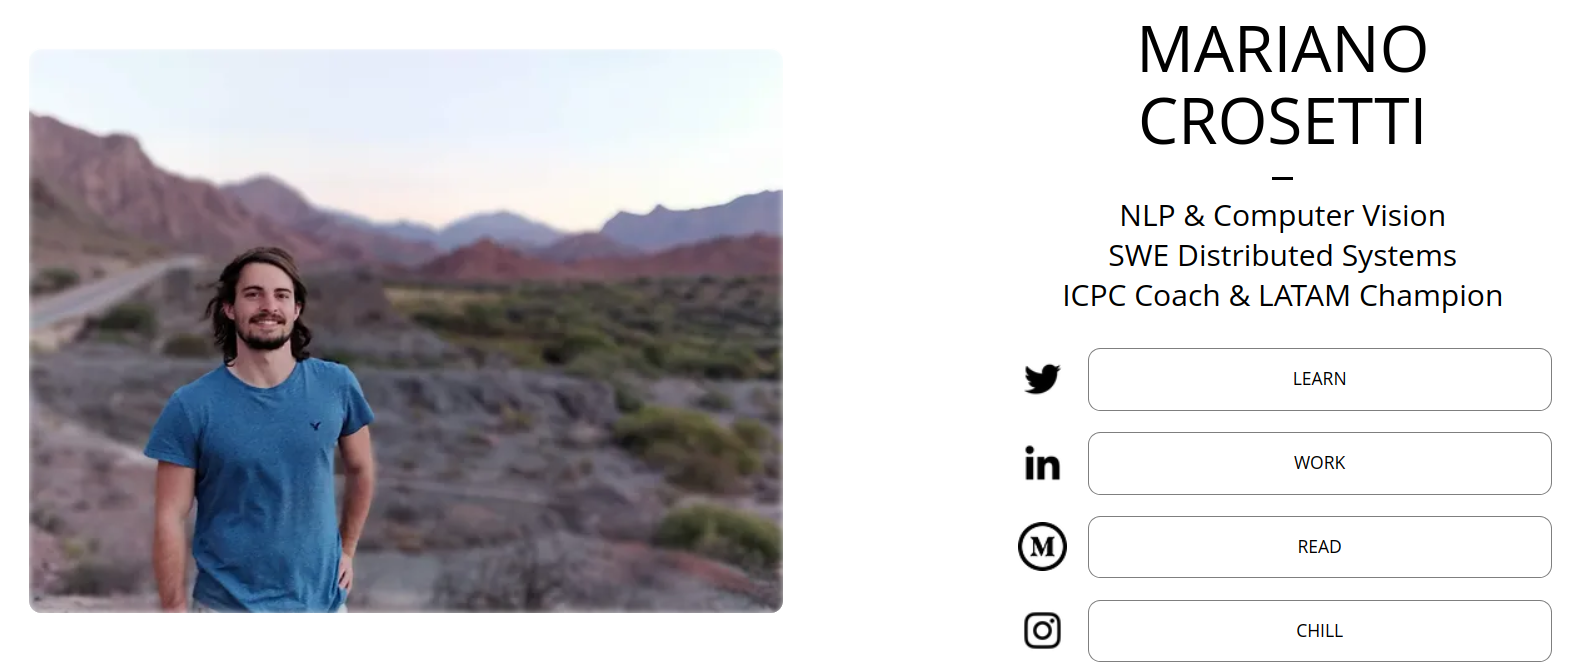
\includegraphics[scale=0.22]{mcros.png}
  \end{center}
  \begin{itemize}
    \item [DESCRIPCION BREVE DE LA FIGURA O GRAFICO]
  \end{itemize}
\end{frame}

\begin{frame}{Ejemplo de columnas}
  \begin{columns}
    \begin{column}{0.48\textwidth}
      \begin{itemize}
        \item [PUNTO COLUMNA IZQUIERDA 1]
        \item [PUNTO COLUMNA IZQUIERDA 2]
      \end{itemize}
    \end{column}
    \begin{column}{0.48\textwidth}
      \begin{itemize}
        \item [PUNTO COLUMNA DERECHA 1]
        \item [PUNTO COLUMNA DERECHA 2]
      \end{itemize}
    \end{column}
  \end{columns}
\end{frame}

\end{document}


